\fenicschapter{Electromagnetic Waveguide Analysis}
              {Electromagnetic Waveguide Analysis}
              {Evan Lezar and David B. Davidson}
              {lezar}

%------------------------------------------------------------------------------
\newcommand{\curl}[2]{\nabla_{#2} \times {#1}}
%
\newcommand{\intoverdomain}[2]{\int_{#2}{#1}{d#2}}
%
\newcommand{\twobytwo}[4]{\begin{bmatrix} #1 & #2\\#3 & #4\end{bmatrix}}
\newcommand{\twobyone}[2]{\begin{Bmatrix}#1\\#2\end{Bmatrix}}

\editornote{Reduce the number of macros.}

% Introduction
At their core, Maxwell's equations\index{Maxwell's equations} are a
set of differential equations describing the interactions between
electric and magnetic fields, charges, and currents. These equations
provide the tools with which to predict the behaviour of
electromagnetic phenomena\index{electromagnetics}, giving us the
ability to use them in a wide variety of applications, including
communication and power generation. Due to the complex nature of
typical problems in these fields, numeric methods such as the finite
element method are often employed to solve them.

One of the earliest applications of the finite element method in
electromagnetics was in waveguide\index{waveguide}
analysis~\cite{Davidson2005}. Since waveguides are some of the most common
structures in microwave engineering, especially in areas where high
power and low loss are essential~\cite{Pozar2005}, their analysis is
still a topic of much interest. This chapter considers the use of
\fenics{} in the cutoff and dispersion analysis of these structures as
well as the analysis of waveguide discontinuities. These types of
analysis form an important part of the design and optimisation of
waveguide structures for a particular purpose.

The aim of this chapter is to guide the reader through the process
followed in implementing solvers for various electromagnetic problems
with both cutoff and dispersion analysis considered in depth. To this
end a brief introduction of electromagnetic waveguide theory, the
mathematical formulation of these problems, and the specifics of their
solution using the finite element method are presented in
\ref{lezar:sec:formulation}. This lays the groundwork for a discussion of
the details pertaining to the \fenics{} implementation of these
solvers, covered in \ref{lezar:sec:Implementation}. The translation of the
finite element formulation to \fenics{}, as well as some
post-processing considerations are covered. In \ref{lezar:sec:Examples} the
solution results for three typical waveguide configurations are
presented and compared to analytical or previously published data.
This serves to validate the implementation and illustrates the kinds
of problems that can be solved. Results for the analysis of H-plane
waveguide discontinuities are then presented in
\ref{lezar:sec:waveguide_discontinuities} with two test cases being
considered.

%------------------------------------------------------------------------------
\section{Formulation}
\label{lezar:sec:formulation}

As mentioned, in electromagnetics, the behaviour of the electric and
magnetic fields are described by Maxwell's equations~\cite{Jin2002,
Smi1997}.  Using these partial differential equations, various
boundary value problems can be obtained depending on the problem being
solved.  In the case of time-harmonic fields, the equation used is the
vector Helmholtz\index{vector Helmholtz equation} wave equation. If
the problem is further restricted to a domain surrounded by perfect
electrical or magnetic conductors (as is the case in general waveguide
problems) the wave equation in terms of the electric field, $\mathbf{E}$, can
be written as~\cite{Jin2002}
\begin{equation}
    \label{lezar:eqn:vector_helmholtz}
    \curl{\frac{1}{\mu_r}\curl{\mathbf{E}}{}}{} - k_o^2\epsilon_r\mathbf{E} = 0, \text{ in
    $\Omega$},
\end{equation}
subject to the boundary conditions
\begin{align}
    \label{lezar:eqn:electric_wall_BC}
    \hat{\mathbf{n}}\times\mathbf{E} &= 0 \text{ on $\Gamma_{e}$}\\
    \label{lezar:eqn:magnetic_wall_BC}
    \hat{\mathbf{n}}\times\curl{\mathbf{E}}{} &= 0 \text{ on $\Gamma_{m}$},
\end{align}
with $\Omega$ representing the interior of the waveguide and
$\Gamma_{e}$ and $\Gamma_{m}$ electric and magnetic walls
respectively. $\mu_r$ and $\epsilon_r$ are the relative magnetic permeability
and electric permittivity respectively.  These are material parameters
that may be position dependent but only the isotropic case is
considered here. $k_o$ is the operating
wavenumber\index{wavenumber!operating} which is related to the
operating frequency ($f_o$) by the expression
\begin{equation}
 k_o = \frac{2\pi f_o}{c_0},
\end{equation}
with $c_0$ the speed of light in free space.  This boundary value
problem (BVP) can also be written in terms of the magnetic
field~\cite{Jin2002}, but as the discussions following are applicable
to both formulations this will not be considered here.

If the guide is sufficiently long, and the $z$-axis is chosen parallel
to its central axis as shown in Figure \ref{lezar:fig:long_waveguide}, then
$z$-dependence of the electric field can be assumed to be of the form
$e^{-\gamma z}$ with $\gamma = \alpha + j\beta$ a complex
propagation\index{propagation constant} constant~\cite{PelosiCoccioliSelleri1998,
Poz2005}.  Making this assumption and splitting the electric field
into transverse ($\mathbf{E}_t$) and axial ($\hat{\mathbf{z}}E_z$) components,
results in the following expression for the field
\begin{equation}
    \label{lezar:eqn:field_components}
    \mathbf{E}(x,y,z) = [\mathbf{E}_t(x,y) + \hat{\mathbf{z}}E_z(x,y)]e^{-\gamma z},
\end{equation}
with $x$ and $y$ the Cartesian coordinates in the cross-sectional plane of the
waveguide and $z$ the coordinate along the length of the waveguide.

\begin{figure}
 \centering
 %\psfrag{x}[b1][1][2][0]{$x$}
 %\psfrag{y}[b1][1][2][0]{$y$}
 %\psfrag{z}[b1][1][2][0]{$z$}
 %\psfrag{G}[b1][1][2][0]{$\Gamma_{e}$}
 %\psfrag{domain}[b1][1][2][0]{$\Omega$}
 \resizebox{0.55\textwidth}{!}{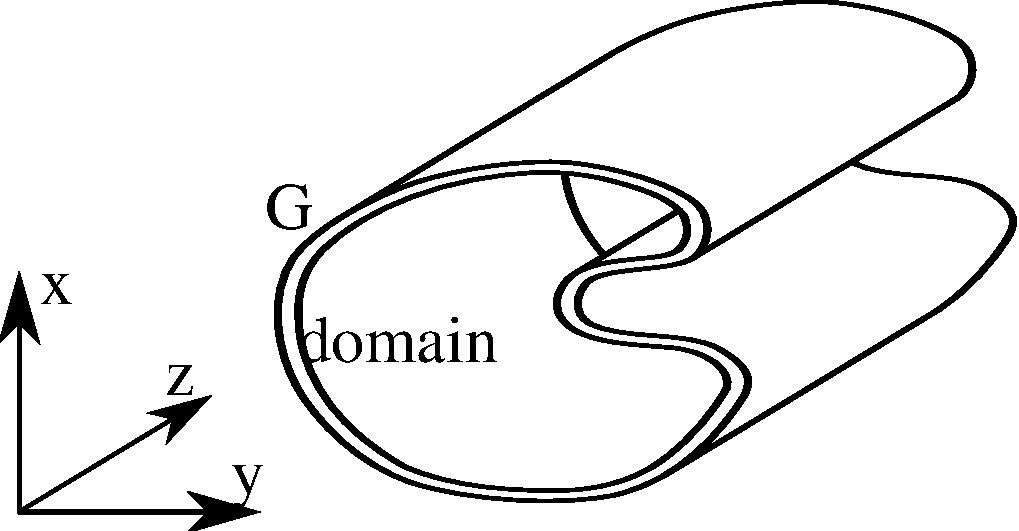
\includegraphics{chapters/lezar/pdf/arbitrary_waveguide_cross_section.pdf}}
 \caption{A long waveguide with an arbitrary cross-section aligned with the $z$-axis.}
 \label{lezar:fig:long_waveguide}
\end{figure}

From \eqref{lezar:eqn:field_components} as well as the BVP described by
\eqref{lezar:eqn:vector_helmholtz}, \eqref{lezar:eqn:electric_wall_BC}, and
\eqref{lezar:eqn:magnetic_wall_BC} it is possible to obtain the following
variational functional found in many computational electromagnetic
texts
\cite{Jin2002, PelCoc1998}
\begin{multline}
    \label{lezar:eqn:functional}
    F(\mathbf{E}) = \frac{1}{2}\int_{\Omega}\frac{1}{\mu_r}(\curl{\mathbf{E}_t}{t})\cdot(\curl{\mathbf{E}_t}{t}) -k_o^2\epsilon_r\mathbf{E}_t\cdot{\mathbf{E}_t}\\
    +\frac{1}{\mu_r}(\nabla_t{E_z} + \gamma\mathbf{E}_t)\cdot(\nabla_t{E_z} + \gamma\mathbf{E}_t)
    -k_o^2\epsilon_r E_z{E_z} d\Omega,
\end{multline}
with
\begin{equation}
    \nabla_t = \frac{\partial}{\partial x}\hat{\mathbf{x}} + \frac{\partial}{\partial
    y}\hat{\mathbf{y}}
\end{equation}
the transverse del operator.

A number of other approaches have also been taken to this
problem. Some, for instance, involve only nodal based elements; some
use the longitudinal fields as the working variable, and the problem
has also been formulated in terms of potentials, rather than fields. A
good summary of these may be found in Chapter 9 of \cite{ZhuCan2006}. The approach used here, involving transverse and
longitudinal fields, is probably the most widely used in practice.

\subsection{Waveguide Cutoff Analysis}
\label{lezar:sec:cutoff_formulation}
\index{waveguide!cutoff analysis}
One of the simplest cases to consider, and often a starting point when
testing a new finite element implementation, is waveguide cutoff
analysis. When a waveguide is operating at cutoff, the electric field
is uniform along the $z$-axis which corresponds with $\gamma = 0$ in
\eqref{lezar:eqn:field_components}~\cite{Pozar2005}.  Substituting $\gamma = 0$ into
\eqref{lezar:eqn:functional} yields the following functional
\begin{multline}
    \label{lezar:eqn:functional_cutoff}
    F(\mathbf{E}) = \frac{1}{2}\int_{\Omega}\frac{1}{\mu_r}(\curl{\mathbf{E}_t}{t})\cdot(\curl{\mathbf{E}_t}{t}) -k_c^2\epsilon_r\mathbf{E}_t\cdot{\mathbf{E}_t}\\
    +\frac{1}{\mu_r}(\nabla_t{E_z})\cdot(\nabla_t{E_z})
    -k_c^2\epsilon_r E_z{E_z} d\Omega.
\end{multline}
The symbol for the operating wavenumber\index{wavenumber!operating}
$k_o$ has been replaced with $k_c$, indicating that the
quantity of interest is now the cutoff
wavenumber\index{wavenumber!cutoff}. This quantity in addition to the
field distribution at cutoff are of interest in these kinds of
problems.  Using two dimensional vector basis functions for the
discretisation of the transverse field, and scalar basis functions for
the axial components, the minimisation of
\eqref{lezar:eqn:functional_cutoff} is equivalent to solving the following
matrix equation
\begin{equation}
    \label{lezar:eqn:matrix_equation_cutoff}
    \begin{bmatrix} S_{tt} & 0\\0 &
    S_{zz}\end{bmatrix}\begin{Bmatrix}e_t\\e_z\end{Bmatrix} =
    k_c^2\begin{bmatrix} T_{tt} & 0\\0 &
    T_{zz}\end{bmatrix}\begin{Bmatrix}e_t\\e_z\end{Bmatrix},
\end{equation}
which is in the form of a general eigenvalue problem\index{eigenvalue
problem}.  Here $S_{ss}$ and $T_{ss}$ represents the stiffness and
mass common to finite element literature~\cite{Davidson2005, Jin2002} with
the subscripts $_{tt}$ and $_{zz}$ indicating transverse or axial
components respectively.  The entries of the matrices of
\eqref{lezar:eqn:matrix_equation_cutoff} are defined as
\begin{align}
\label{lezar:eqn:s_tt_ij}
(s_{tt})_{ij} &= \intoverdomain{\frac{1}{\mu_r}(\curl{\mathbf{N}_i}{t})\cdot(\curl{\mathbf{N}_j}{t})}{\Omega},\\
\label{lezar:eqn:t_tt_ij}
(t_{tt})_{ij} &= \intoverdomain{\epsilon_r\mathbf{N}_i\cdot\mathbf{N}_j}{\Omega},\\
\label{lezar:eqn:s_zz_ij}
(s_{zz})_{ij} &= \intoverdomain{\frac{1}{\mu_r}(\nabla_t{M_i})\cdot(\nabla_t{M_j})}{\Omega},\\
\label{lezar:eqn:t_zz_ij}
(t_{zz})_{ij} &= \intoverdomain{\epsilon_r M_i M_j}{\Omega},
\end{align}
with $\intoverdomain{}{\Omega}$ representing integration over the
cross-section of the waveguide and $\mathbf{N}_i$ and $M_i$
representing the $i^{\text{th}}$ vector and scalar basis functions
respectively.

Due to the block nature of the matrices the eigensystem can be written
as two smaller systems
\begin{align}
    \begin{bmatrix}S_{tt}\end{bmatrix}\begin{Bmatrix}e_t\end{Bmatrix} &=
    k_{c,TE}^{2}\begin{bmatrix}
    T_{tt}\end{bmatrix}\begin{Bmatrix}e_t\end{Bmatrix},\\
    \begin{bmatrix}S_{zz}\end{bmatrix}\begin{Bmatrix}e_z\end{Bmatrix} &= k_{c,TM}^{2}\begin{bmatrix}T_{zz}\end{bmatrix}\begin{Bmatrix}e_z\end{Bmatrix},
\end{align}
with $k_{c,TE}$ and $k_{c,TM}$ corresponding to the cutoff
wavenumbers\index{wavenumber!cutoff} of the transverse electric ($TE$)
and transverse magnetic ($TM$) modes respectively. The eigenvectors
($\{e_t\}$ and $\{e_z\}$) of the systems are the coefficients of the
vector and scalar basis functions, allowing for the calculation of the
transverse and axial field distributions associated with a waveguide
cutoff mode.

\subsection{Waveguide Dispersion Analysis}
\label{lezar:sec:propagation_curves}
\index{waveguide!dispersion analysis}
In the case of cutoff analysis discussed in
\ref{lezar:sec:cutoff_formulation}, one attempts to obtain the value of
$k_o^2 = k_c^2$ for a given propagation constant $\gamma$,
namely $\gamma = 0$.  For most waveguide design applications however,
$k_o$ is specified and the propagation constant is calculated
from the resultant eigensystem~\cite{Jin2002, PelCoc1998}.  This
calculation can be simplified somewhat by making the following
substitution into \eqref{lezar:eqn:functional}
\begin{equation}
    \mathbf{E}_{t,\gamma} = \gamma\mathbf{E}_t,
\end{equation}
which results in the modified functional
\begin{multline}
    \label{lezar:eqn:functional_scaled}
    F(\mathbf{E}) =
    \frac{1}{2}\int_{\Omega}\frac{1}{\mu_r}(\curl{\mathbf{E}_{t,\gamma}}{t})\cdot(\curl{\mathbf{E}_{t,\gamma}}{t}) -k_o^2\epsilon_r\mathbf{E}_{t,\gamma}\cdot{\mathbf{E}_{t,\gamma}}\\
    -\gamma^2\left[\frac{1}{\mu_r}(\nabla_t{E_z} +
    \mathbf{E}_{t,\gamma})\cdot(\nabla_t{E_z} + \mathbf{E}_{t,\gamma})-k_o^2\epsilon_r
    E_z{E_z}\right] d\Omega.
\end{multline}
Using the same discretisation as for cutoff analysis discussed in \ref{lezar:sec:cutoff_formulation}, the matrix equation associated with the solution of the variational problem is given by
\begin{equation}
    \label{lezar:eqn:matrix_equation_dispersion}
    \begin{bmatrix} A_{tt} & 0\\0 & 0\end{bmatrix}\begin{Bmatrix}e_t\\e_z\end{Bmatrix} =
    \gamma^2\begin{bmatrix} B_{tt} & B_{tz}\\B_{zt} &
    B_{zz}\end{bmatrix}\begin{Bmatrix}e_t\\e_z\end{Bmatrix},
\end{equation}
with
\begin{align}
    A_{tt} = S_{tt} - k_o^2 T_{tt},\\
    B_{zz} = S_{zz} - k_o^2 T_{zz},
\end{align}
which is in the form of a generalised eigenvalue
problem\index{eigenvalue problem} with the eigenvalues corresponding
to the square of the complex propagation constant ($\gamma$).

The matrices $S_{tt}$, $T_{tt}$, $S_{zz}$, and $T_{zz}$ are identical
to those defined in \ref{lezar:sec:cutoff_formulation} with entries given by
\eqref{lezar:eqn:s_tt_ij}, \eqref{lezar:eqn:t_tt_ij}, \eqref{lezar:eqn:s_zz_ij}, and \eqref{lezar:eqn:t_zz_ij} respectively.
The entries of the other sub-matrices, $B_{tt}$, $B_{tz}$, and
$B_{zt}$, are defined by
\begin{align}
(b_{tt})_{ij} &=
\intoverdomain{\frac{1}{\mu_r}\mathbf{N}_i\cdot\mathbf{N}_j}{\Omega},\\
(b_{tz})_{ij} &=
\intoverdomain{\frac{1}{\mu_r}\mathbf{N}_i\cdot\nabla_t{M_j}}{\Omega},\\
(b_{zt})_{ij} &=
\intoverdomain{\frac{1}{\mu_r}\nabla_t{M_i}\cdot\mathbf{N}_j}{\Omega}.
\end{align}

A common challenge in electromagnetic eigenvalue problems such as
these is the occurrence of spurious
modes~\cite{Davidson2005}\index{spurious modes}.  These are non-physical
modes that fall in the null space of the $\curl{\curl{}{}}{}$ operator
of \eqref{lezar:eqn:vector_helmholtz}~\cite{Bossavit1998} (The issue of spurious
modes is not as closed as most computational electromagnetics texts
indicate. For a summary of recent work in the applied mathematics
literature, written for an engineering readership,
see~\cite{FernandesRaffetto2002}).

One of the strengths of the vector basis functions used in the
discretisation of the transverse component of the field is that it
allows for the identification of these spurious modes~\cite{Davidson2005,
Jin2002}.  In~\cite{LeeSunCendes1991} a scaling method is proposed to shift
the eigenvalue spectrum such that the dominant waveguide mode (usually
the lowest non-zero eigenvalue) corresponds with the largest
eigenvalue of the new system. Other approaches have also been followed
to address the spurious modes. In~\cite{VardapetyanDemkowicz2002}, Lagrange
mutipliers are used to move these modes from zero to infinity.

In the case of the eigensystem associated with dispersion analysis,
the matrix equation of \eqref{lezar:eqn:matrix_equation_dispersion} is
scaled as follows
\begin{equation}
    \label{lezar:eqn:matrix_equation_dispersion_scaled}
    \twobytwo{B_{tt}}{B_{tz}}{B_{zt}}{B_{zz}}\twobyone{e_t}{e_z} =
    \frac{\theta^2}{\theta^2 +
    \gamma^2}\twobytwo{B_{tt} +
    \frac{A_{tt}}{\theta^2}}{B_{tz}}{B_{zt}}{B_{zz}}\twobyone{e_t}{e_z},
\end{equation}
with $\theta^2 = k_o^2\mu_r^{(max)}\epsilon_r^{(max)}$ an upper bound on
the square of the propagation constant ($\gamma^2$) and $\mu_r^{(max)}$
and $\epsilon_r^{(max)}$ the maximum relative permeability and permittivity
in the computational domain.

If $\lambda$ is an eigenvalue of the scaled system of
\eqref{lezar:eqn:matrix_equation_dispersion_scaled}, then the propagation constant can be
calculated as
\begin{equation}
    \gamma^2 = \frac{1 - \lambda}{\lambda}\theta^2,
\end{equation}
and thus $\gamma^2 \rightarrow \infty$ as $\lambda \rightarrow 0$, which moves the spurious modes out of the region of interest.

\section{Implementation}
\label{lezar:sec:Implementation}

This section considers the details of the implementation of
a \fenics-based solver for waveguide cutoff mode and dispersion curve
problems as described in \ref{lezar:sec:cutoff_formulation}
and \ref{lezar:sec:propagation_curves}. A number of code snippets
illustrate some of the finer points of the implementation.

\subsection{Formulation}
\lstlistingname{}~\ref{lezar:listing:function_spaces} shows the definitions of the function spaces used in the solution of the problems considered here. \nedelec{} basis functions of the first kind ({\tt N\_v} and {\tt N\_u}) are used to approximate the transverse component of the electric field. This ensures that the tangential continuity required at element and material boundaries can be enforced~\cite{Jin2002}.  The axial component of the field is modelled using a set of Lagrange basis functions ({\tt M\_v}, and {\tt M\_u}). Additionally, a discontinuous Galerkin function space is included to allow for the modelling of material parameters such as dielectrics.
\begin{python}
V_DG = FunctionSpace(mesh, "DG", 0)
V_N = FunctionSpace(mesh, "Nedelec 1st kind H(curl)", transverse_order)
V_M = FunctionSpace(mesh, "Lagrange", axial_order)

combined_space = V_N * V_L

(N_v, M_v) = TestFunctions(combined_space)
(N_u, M_u) = TrialFunctions(combined_space)
\end{python}

In order to deal with material properties, the {\tt Expression} class is
subclassed and the {\tt eval()} method overridden. This is illustrated
in \lstlistingname{} \ref{lezar:listing:material_properties} where a
dielectric with a relative permittivity of $\epsilon_r = 4$ that extends to
$y = 0.25$ is shown. This class is then instantiated using the
discontinuous Galerkin function space already discussed. For constant
material properties (such as the inverse of the magnetic permittivity
$\mu_r$, in this case) a JIT-compiled expression is used.

\begin{python}
class HalfLoadedDielectric(Expression):
    def eval(self, values, x):
        if x[1] < 0.25:
            values[0] = 4.0
        else:
            values[0] = 1.0;

e_r = HalfLoadedDielectric(V_DG)
one_over_u_r = Expression("1.0")

k_o_squared = Expression("value", {"value" : 0.0})
theta_squared = Expression("value", {"value" : 0.0})
\end{python}

The basis functions declared in \lstlistingname{}
 \ref{lezar:listing:function_spaces} and the desired material property
 functions are now used to create the forms required for the matrix
 entries specified in \ref{lezar:sec:cutoff_formulation} and
 \ref{lezar:sec:propagation_curves}. The forms are shown in
 \lstlistingname{} \ref{lezar:listing:forms} and the matrices of
 \eqref{lezar:eqn:matrix_equation_cutoff},
 \eqref{lezar:eqn:matrix_equation_dispersion}, and
 \eqref{lezar:eqn:matrix_equation_dispersion_scaled} can be assembled using
 the required combinations of these forms with the right hand side of
 \eqref{lezar:eqn:matrix_equation_dispersion_scaled}, {\tt rhs}, provided as
 an example.  It should be noted that the use of JIT-compiled expressions for
 operating wavenumber and scaling parameters means that the forms need
 not be recompiled each time the operating frequency is changed. This
 is especially beneficial when the calculation of dispersion curves is
 considered since the same calculation is performed for a range of
 operating frequencies.

\begin{python}
s_tt = one_over_u_r*dot(curl_t(N_v), curl_t(N_u))
t_tt = e_r*dot(N_v, N_u)

s_zz = one_over_u_r*dot(grad(M_v), grad(M_u))
t_zz = e_r*M_v*M_u

b_tt = one_over_u_r*dot(N_v, N_u)
b_tz = one_over_u_r*dot(N_v, grad(M_u))
b_zt = one_over_u_r*dot(grad(M_v), N_u)

a_tt = s_tt - k_o_squared*t_tt
b_zz = s_zz - k_o_squared*t_zz

rhs = b_tt + b_tz + b_zt + b_zz + 1.0/theta_squared*a_tt
\end{python}

From \eqref{lezar:eqn:electric_wall_BC} it follows that the tangential
component of the electric field must be zero on perfectly electrical
conducting (PEC) surfaces. What this means in practice is that the
degrees of freedom associated with both the Lagrange and \nedelec{}
basis functions on the boundary must be set to zero since there can be
no electric field inside a perfect electrical
conductor~\cite{Smith1997}. An example for a PEC surface surrounding the
entire computational domain is shown in \lstlistingname{}
\ref{lezar:listing:boundary_conditions} as the {\tt ElectricWalls}
class. This boundary condition can then be applied to the constructed
matrices before solving the eigenvalue systems.

The boundary condition given in \eqref{lezar:eqn:magnetic_wall_BC} results
in a natural boundary condition for the problems considered and thus
it is not necessary to explicitly enforce it~\cite{PelosiCoccioliSelleri1998}.  Such
magnetic walls and the symmetry of a problem are often used to
decrease the size of the computational domain although this does limit
the solution obtained to even modes~\cite{Jin2002}.

\begin{python}
class ElectricWalls(SubDomain):
    def inside(self, x, on_boundary):
        return on_boundary

zero = Expression(("0.0","0.0","0.0")
dirichlet_bc = DirichletBC(combined_space, zero, ElectricWalls())
\end{python}

Once the required matrices have been assembled and the boundary
conditions applied, the resultant eigenproblem can be solved. This can
be done by outputting the matrices and solving the problem externally,
or by making use of the eigensolvers provided by SLEPc that can be
integrated into the \fenics{} package.

\subsection{Post-Processing}

After the eigenvalue system has been solved and the required eigenpair
chosen, this can be post-processed to obtain various quantities of
interest. For the cutoff wavenumber\index{wavenumber!cutoff}, this is
a relatively straight-forward process and only involves simple
operations on the eigenvalues of the system. For the calculation of
dispersion curves and visualisation of the resultant field components
the process is slightly more complex.

\paragraph{Dispersion Curves}
\index{dispersion curves}

For dispersion curves the computed value of the propagation constant
($\gamma$) is plotted as a function of the operating frequency
($f_o$).  Since $\gamma$ is a complex variable, a mapping is required
to represent the data on a single two-dimensional graph. This is
achieved by choosing the $f_o$-axis to represent the value $\gamma =
0$, effectively dividing the {$\gamma-f_o$} plane into two
regions. The region above the $f_o$-axis is used to represent the
magnitude of the imaginary part of $\gamma$, whereas the real part
falls in the lower region. A mode that propagates along the guide for
a given frequency will thus lie in the upper half-plane of the plot
and a complex mode will be represented by a data point above and below
the $f_o$-axis.  This procedure is followed in~\cite{PelosiCoccioliSelleri1998} and
other literature and allows for quick comparisons and validation of
results.

\paragraph{Field Visualisation}

In order to visualise the fields associated with a given solution, the
basis functions need to be weighted with coefficients corresponding to
the entries in an eigenvector obtained from one of the eigenvalue
problems. In addition, the transverse or axial components of the field
may need to be extracted. An example for plotting the transverse and
axial components of the field is given in \lstlistingname{}
\ref{lezar:listing:field_component_visualisation}.  Here the variable {\tt
x} assigned to the function vector is one of the eigenvectors obtained
by solving the eigenvalue problem.

\begin{python}
f = Function(combined_space, x)

(transverse, axial) = f.split()

plot(transverse)
plot(axial)
\end{python}

The {\tt eval()} method of the {\tt transverse} and {\tt axial}
functions can also be called in order to evaluate the functions at a
given spatial coordinate, allowing for further visualisation or
post-processing options.

\section{Examples}
\label{lezar:sec:Examples}

The first of the examples considered is the canonical one of a hollow
waveguide, which has been covered in a multitude of texts on the
subject~\cite{Davidson2005, Jin2002, PelCoc1998, Poz2005}.  Since the
analytical solutions for this structure are known, it provides an
excellent benchmark and is a typical starting point for the validation
of a computational electromagnetic solver for solving waveguide
problems.

The second and third examples are a partially filled rectangular guide
and a shielded microstrip line on a dielectric substrate,
respectively. In each case results are compared to published results
from the literature as a means of validation.

\subsection{Hollow Rectangular Waveguide}
\index{waveguide!hollow rectangular|(}

Figure \ref{lezar:fig:hollow_rectangular_guide} shows the cross section of a
hollow rectangular waveguide. For the purpose of this chapter a guide
with dimensions $a = 1\text{m}$ and $b = 0.5\text{m}$ is considered.
\begin{figure}[ht]
    \centering
    %\psfrag{epsilon}{$\epsilon_r = 1$}
    %\psfrag{mu}{$\mu_r = 1$}
    %\psfrag{a}{$a$}
    %\psfrag{b}{$b$}
    \resizebox{0.4\textwidth}{!}{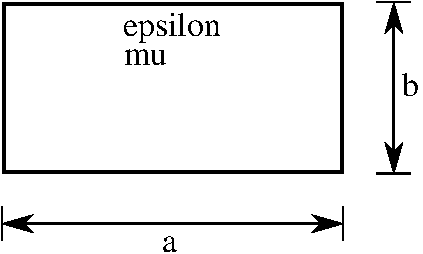
\includegraphics{chapters/lezar/pdf/hollow_rectangular_waveguide.pdf}}
    \caption{A diagram showing the cross section and dimensions of a hollow rectangular waveguide.}
    \label{lezar:fig:hollow_rectangular_guide}
\end{figure}
The analytical expressions for the electric field components of a
hollow rectangular guide with width $a$ and height $b$ are given
by~\cite{Pozar2005}
\begin{align}
    \label{lezar:eqn:rect:E_x analytical}
    E_x &= \frac{n}{b}A_{mn}\cos\left(\frac{m\pi
    x}{a}\right)\sin\left(\frac{n\pi y}{b}\right),\\
    \label{lezar:eqn:rect:E_y analytical}
    E_y &= \frac{-m}{a}A_{mn}\sin\left(\frac{m\pi x}{a}\right)\cos\left(\frac{n\pi y}{b}\right),
\end{align}
for the TE$_{mn}$ mode, whereas the $z$-directed electric field for the TM$_{mn}$ mode has the form~\cite{Pozar2005}
\begin{equation}
 \label{lezar:eqn:rect_E_z_analytical}
 E_z = B_{mn}\sin\left(\frac{m\pi x}{a}\right)\sin\left(\frac{n\pi y}{b}\right),
\end{equation}
with $A_{mn}$ and $B_{mn}$ constants for a given mode.
In addition, the propagation constant, $\gamma$, has the form
\begin{equation}
 \label{lezar:eqn:rectangular_propagation}
 \gamma = \sqrt{k_o^2 - k_c^2},
\end{equation}
with $k_o$ the operating wavenumber dependent on the operating frequency, and
\begin{equation}
 \label{lezar:eqn:rectangular_cutoff}
 k_c^2 = \left(\frac{m\pi}{a}\right)^2 + \left(\frac{n\pi}{b}\right)^2,
\end{equation}
the analytical solution for the square of the cutoff wavenumber\index{wavenumber!cutoff} for both the TE$_{mn}$ and TM$_{mn}$ modes.

\paragraph{Cutoff Analysis}
\index{waveguide!cutoff analysis}

Figure \ref{lezar:fig:rectangular_cutoff_TE} shows the first two calculated
TE cutoff modes for the hollow rectangular guide, with the first two
TM cutoff modes being shown in Figure
\ref{lezar:fig:rectangular_cutoff_TM}. The solution is obtained with 64
triangular elements and second order basis functions in the transverse
as well as the axial discretisations.
\begin{figure}[ht]
\centering
 \subfloat[TE$_{10}$ mode.]{\resizebox{0.45\textwidth}{!}{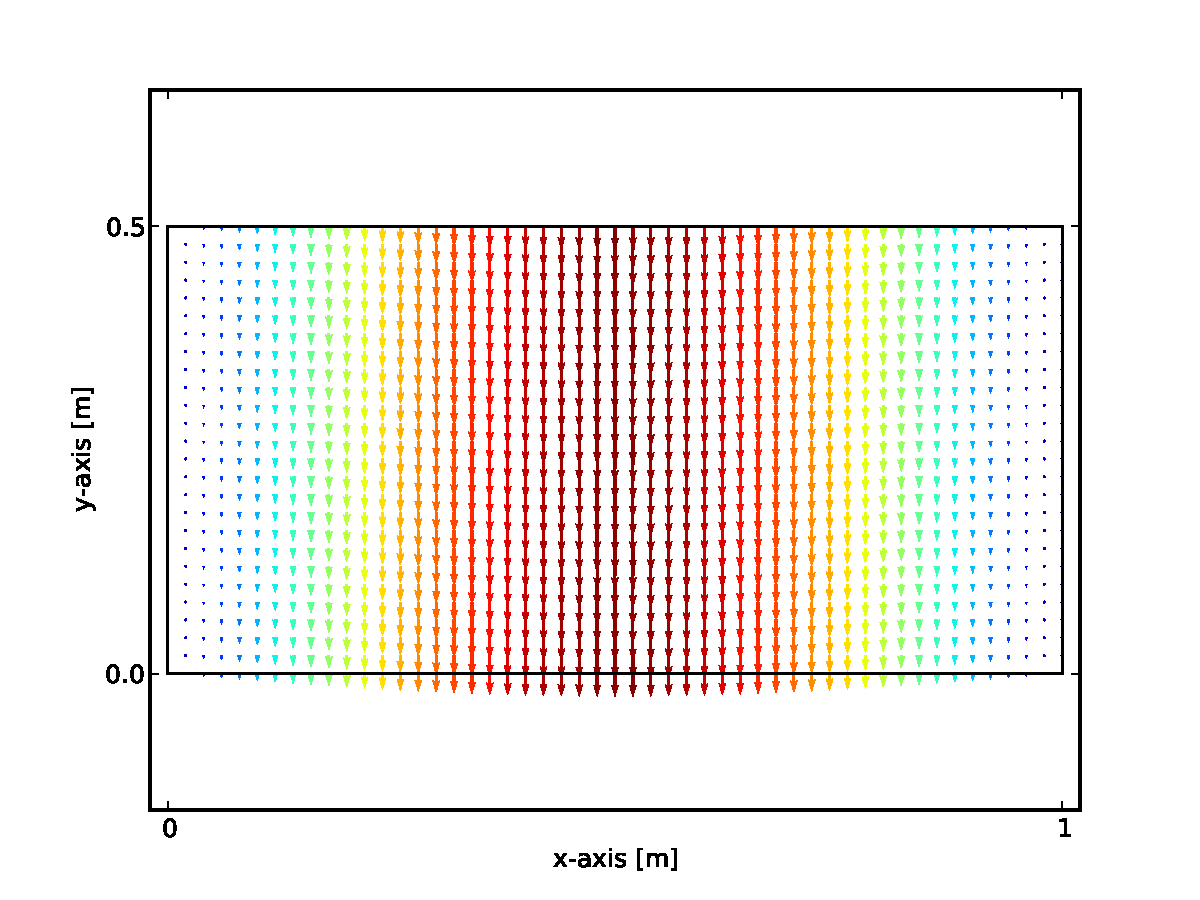
\includegraphics{chapters/lezar/pdf/hollow_rectangular_calculated_TE_10.pdf}}}
 \subfloat[TE$_{01}$ mode.]{\resizebox{0.45\textwidth}{!}{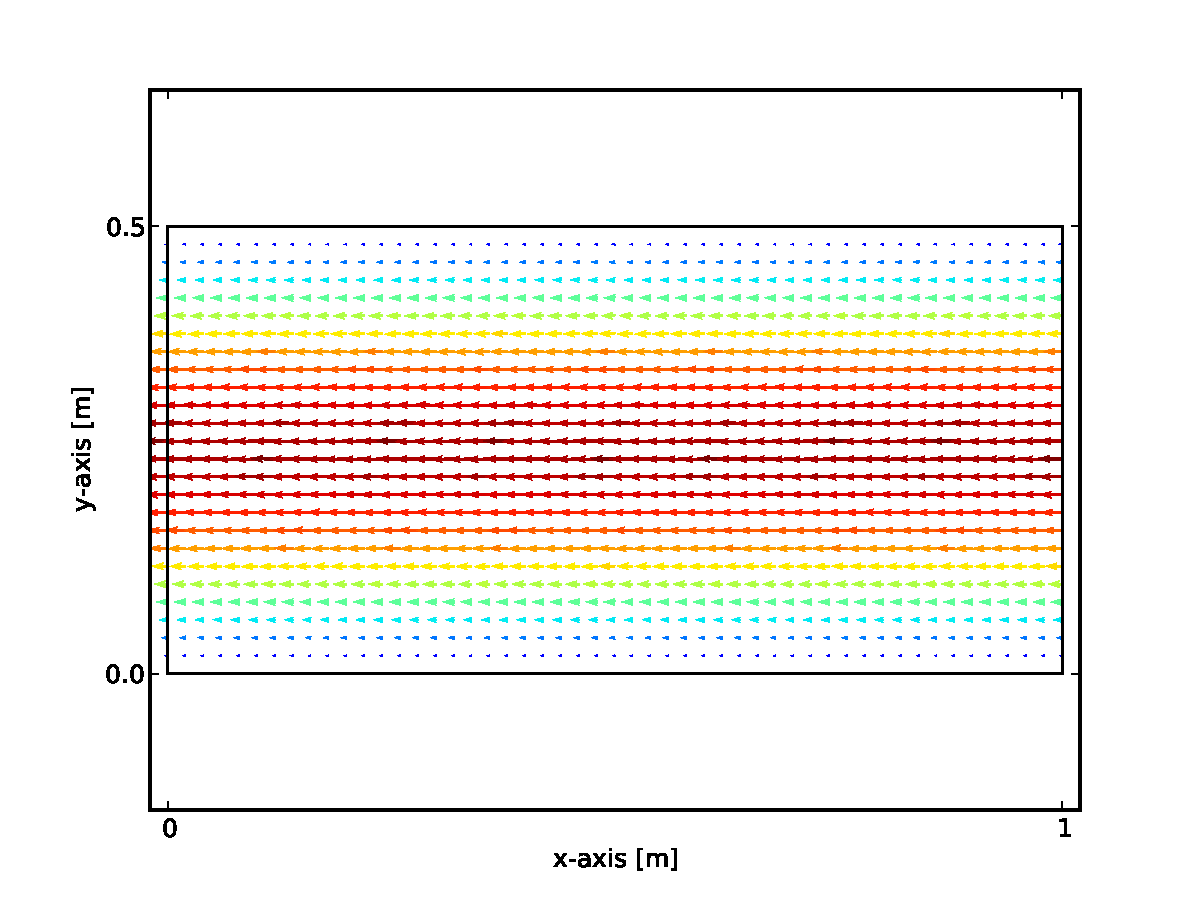
\includegraphics{chapters/lezar/pdf/hollow_rectangular_calculated_TE_01.pdf}}}
\caption{The first two calculated TE cutoff modes of a $1$~m~$\times~0.5$~m hollow rectangular waveguide.}
\label{lezar:fig:rectangular_cutoff_TE}
\end{figure}

\begin{figure}[ht]
\centering
 \subfloat[TM$_{11}$ mode.]{\resizebox{0.45\textwidth}{!}{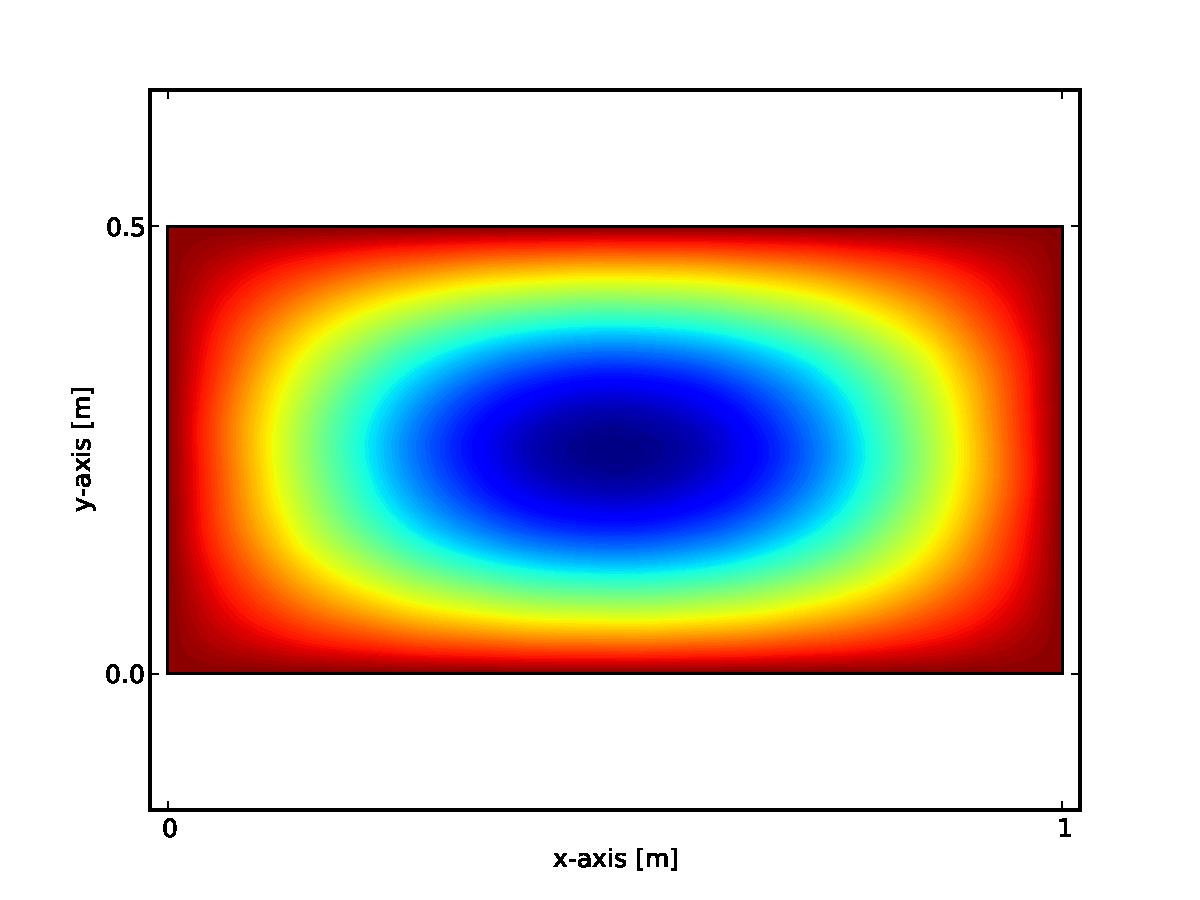
\includegraphics{chapters/lezar/pdf/hollow_rectangular_calculated_TM_11.pdf}}}
 \subfloat[TM$_{21}$ mode.]{\resizebox{0.45\textwidth}{!}{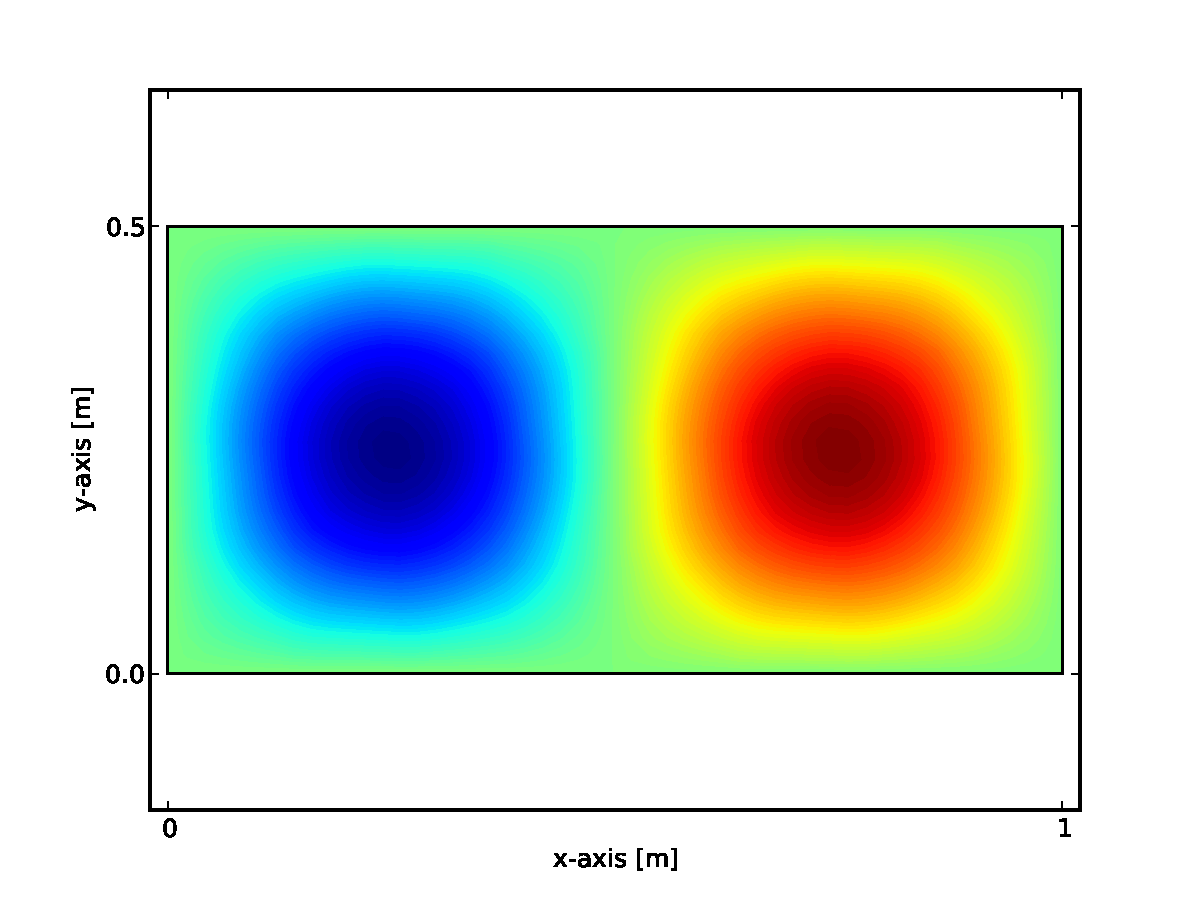
\includegraphics{chapters/lezar/pdf/hollow_rectangular_calculated_TM_21.pdf}}}
\caption{The first two calculated TM cutoff modes of a $1$~m~$\times~0.5$~m hollow rectangular waveguide.}
\label{lezar:fig:rectangular_cutoff_TM}
\end{figure}
Table \ref{lezar:tab:rectangular_cutoff_comparison} gives a comparison of
the calculated and analytical values for the square of the cutoff
wavenumber\index{wavenumber!cutoff} of a number of modes for a hollow
rectangular guide. As can be seen from the table, there is excellent
agreement between the values.

\begin{table}[b]
 \centering
    \caption{Comparison of analytical and calculated cutoff wavenumber squared ($k_c^2$) for various TE and TM modes of a $1$~m~$\times~0.5$~m hollow rectangular waveguide.}
    \label{lezar:tab:rectangular_cutoff_comparison}
    \begin{tabular}{|c|c|c|c|}
    \hline
    Mode & Analytical [m$^{-2}$] & Calculated [m$^{-2}$] & Relative Error \\
    \hline
    TE$_{10}$ & 9.8696 & 9.8696 & 1.4452e-06\\
    TE$_{01}$ & 39.4784 & 39.4784 & 2.1855e-05\\
    TE$_{20}$ & 39.4784 & 39.4784 & 2.1894e-05\\
    \hline
    TM$_{11}$ & 49.3480 & 49.4048 & 1.1514e-03 \\
    TM$_{21}$ & 78.9568 & 79.2197 & 3.3295e-03\\
    TM$_{31}$ & 128.3049 & 129.3059 & 7.8018e-03\\
    \hline
    \end{tabular}
\end{table}
\clearpage
\paragraph{Dispersion Analysis}
\index{waveguide!dispersion analysis}

When considering the calculation of the dispersion curves for the
hollow rectangular waveguide, the mixed formulation as discussed in
\ref{lezar:sec:propagation_curves} is used.  The calculated dispersion
curves for the first 10 modes of the hollow rectangular guide are
shown in Figure~\ref{lezar:fig:hollow_rectangular_dispersion_curves} along
with the analytical results. For the rectangular guide a number of
modes are degenerate with the same dispersion and cutoff properties as
predicted by \eqref{lezar:eqn:rectangular_propagation} and
\eqref{lezar:eqn:rectangular_cutoff}. This explains the visibility of only
six curves. There is excellent agreement between the analytical and
computed results.
\begin{figure}[h]
  \centering
  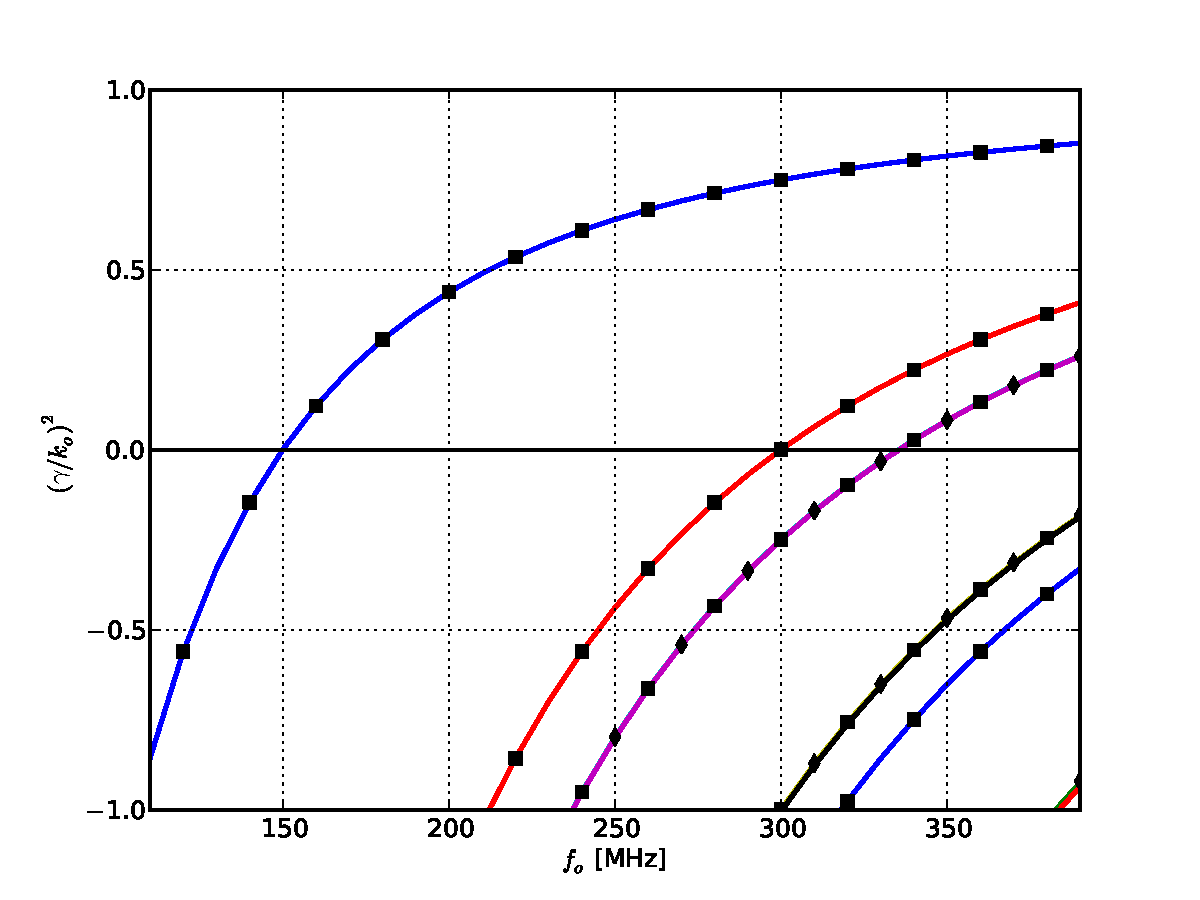
\includegraphics[width=\largefig]{chapters/lezar/pdf/hollow_dispersion_curve.pdf}
  \caption{Dispersion curves for the first 10 modes of a
    $1$~m~$\times~0.5$~m hollow rectangular waveguide. Markers are
    used to indicate the analytical results with $\blacksquare$ and
    $\blacklozenge$ indicating TE and TM modes respectively.}
  \index{dispersion curves}
  \label{lezar:fig:hollow_rectangular_dispersion_curves}
\end{figure}
\index{waveguide!hollow rectangular|)}
\subsection{Half-Loaded Rectangular Waveguide}
\index{waveguide!half-loaded rectangular|(}
In some cases, a hollow rectangular guide may not be the ideal
structure to use due to, for example, limitations on its
dimensions. If the guide is filled with a dielectric material with a
relative permittivty $\epsilon_r > 1$, the cutoff frequency of the dominant
mode will be lowered. Consequently a loaded waveguide will be mode
compact than a hollow guide for the same dominant mode
frequency. Furthermore, in many practical applications, such as
impedance matching or phase shifting sections, a waveguide that is
only partially loaded is used~\cite{Pozar2005}.

Figure~\ref{lezar:fig:half_filled_rectangular_guide} shows the cross section
of such a guide. The guide considered here has the same dimensions as
the hollow rectangular waveguide used in the previous section, but its
lower half is filled with an $\epsilon_r = 4$ dielectric material.
\begin{figure}
    \centering
    %\psfrag{epsilon}{$\epsilon_r = 1$}
    %\psfrag{mu}{$\mu_r = 1$}
    %\psfrag{edielectric}{$\epsilon_r = 4$}
    %\psfrag{a}{$a$}
    %\psfrag{b}{$b$}
    %\psfrag{d}{$d$}
    \resizebox{0.45\textwidth}{!}{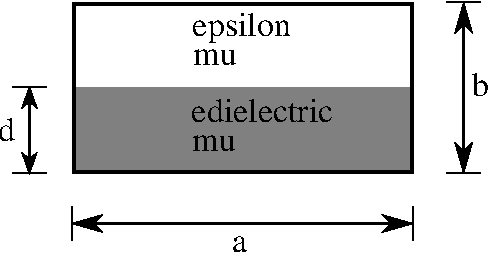
\includegraphics{chapters/lezar/pdf/half_loaded_rectangular_waveguide.pdf}}
    \caption{A diagram showing the cross section and dimensions of a half-loaded rectangular waveguide.  The lower half of the guide is filled with an $\epsilon_r = 4$ dielectric material.}
    \label{lezar:fig:half_filled_rectangular_guide}
\end{figure}

\paragraph{Cutoff Analysis}
\index{waveguide!cutoff analysis}

Figure~\ref{lezar:fig:half_filled_rectangular_cutoff_modes} shows the first
TE and TM cutoff modes of the half-loaded guide shown in
Figure~\ref{lezar:fig:half_filled_rectangular_guide}. Note the concentration
of the transverse electric field in the hollow part of the guide. This
is due to the fact that the displacement flux, $\mathbf{D} =
\epsilon\mathbf{E}$, must be normally continuous at the dielectric
interface~\cite{Pozar2005, Smi1997}.
\begin{figure}[h]
\centering
 \subfloat[First TE mode.]{\resizebox{0.45\textwidth}{!}{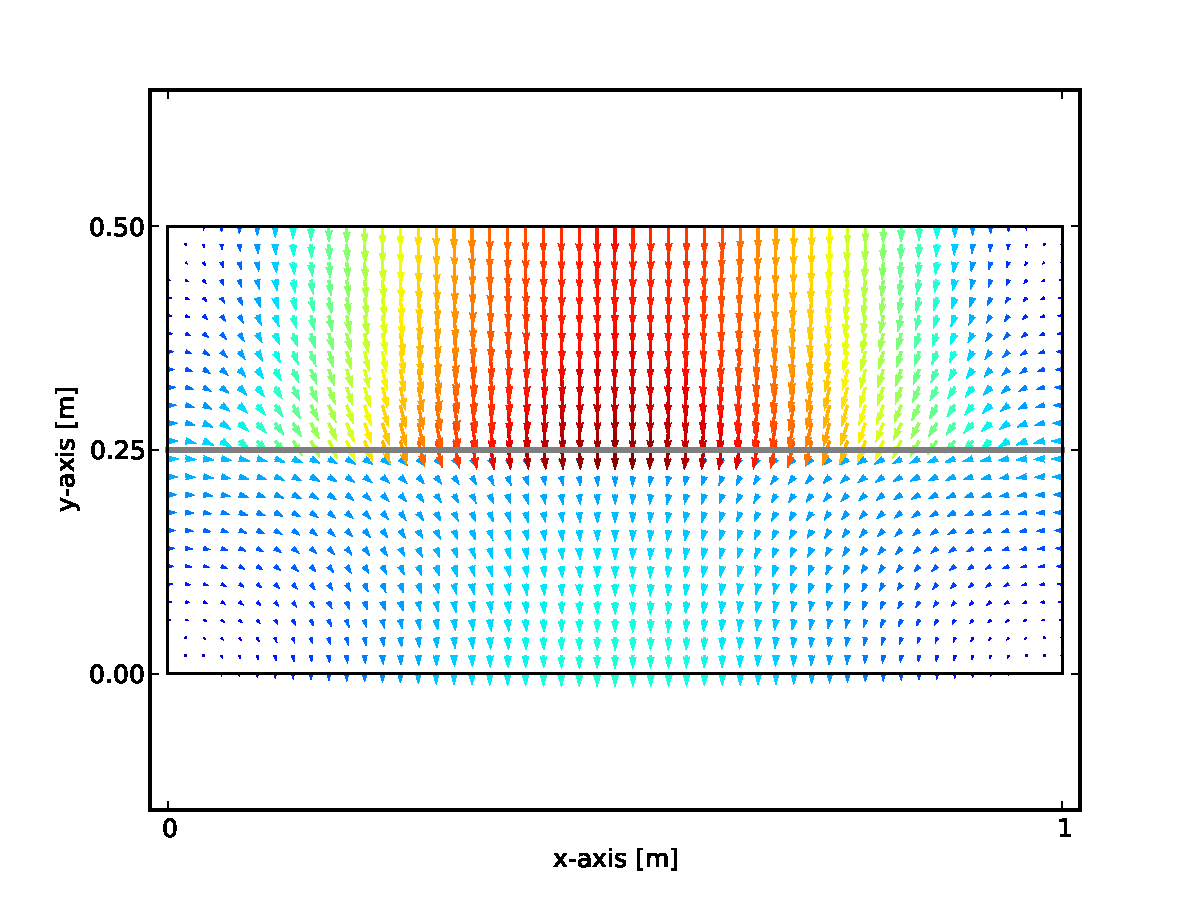
\includegraphics{chapters/lezar/pdf/half_filled_rectangular_calculated_TE_1.pdf}}}
 \subfloat[First TM  mode.]{\resizebox{0.45\textwidth}{!}{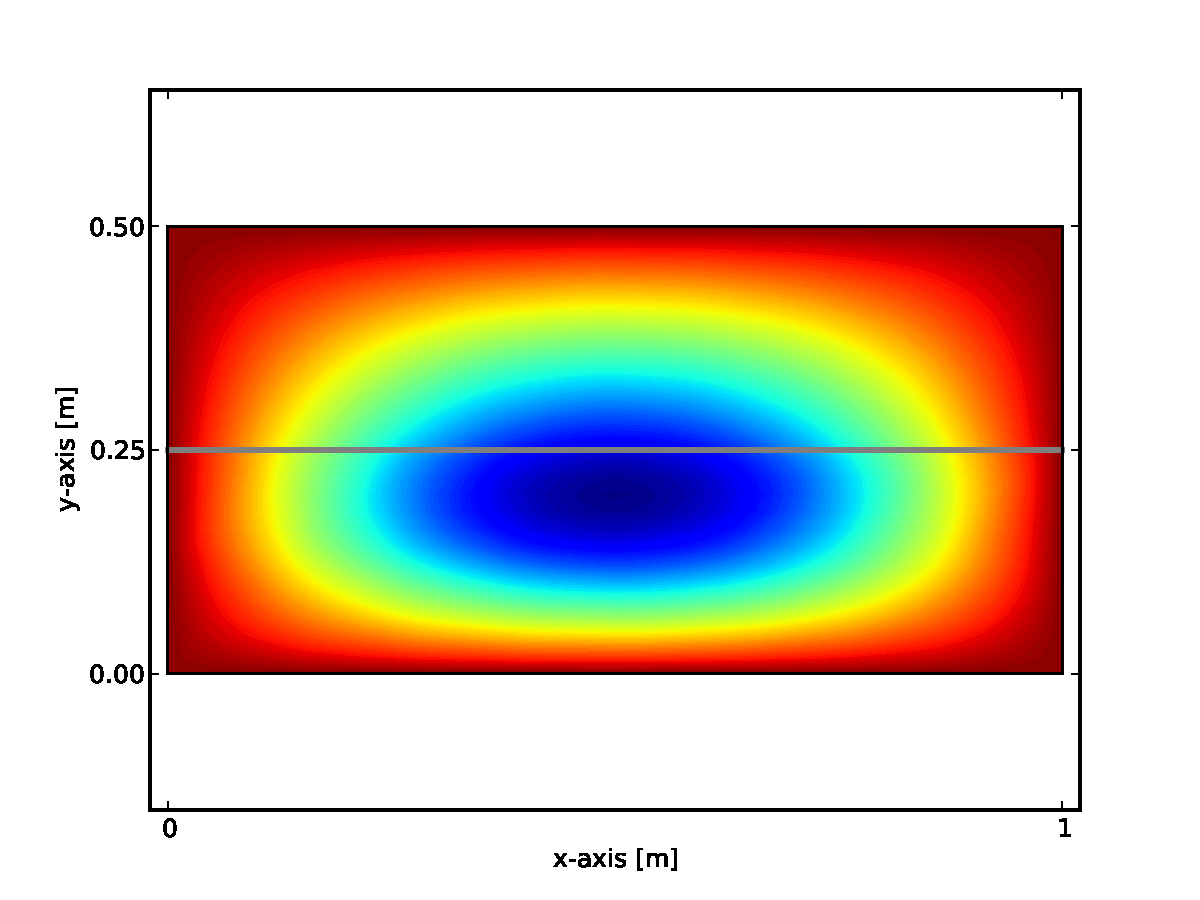
\includegraphics{chapters/lezar/pdf/half_filled_rectangular_calculated_TM_1.pdf}}}
\caption{The first calculated TE and TM cutoff modes of a $1$~m~$\times~0.5$~m rectangular waveguide with the lower half of the guide filled with an $\epsilon_r = 4$ dielectric.}
\label{lezar:fig:half_filled_rectangular_cutoff_modes}
\end{figure}

\paragraph{Dispersion Analysis}
\index{waveguide!dispersion analysis}

The dispersion curves for the first 8 modes of the half-loaded
waveguide are shown in
Figure~\ref{lezar:fig:half_loaded_rectangular_dispersion_curves} with
results for the first 4 modes from~\cite{Jin2002} provided as
reference. Here it can be seen that the cutoff frequency of the
dominant mode has decreased and there is no longer the same degeneracy
in the modes when compared to the hollow guide of the same
dimensions. In addition, there are complex modes present as a result
of the fourth and fifth as well as the sixth and seventh modes
occurring as conjugate pairs at certain points in the spectrum. It
should be noted that the imaginary parts of these conjugate pairs are
very small and thus the $\bullet$ markers in
Figure~\ref{lezar:fig:half_loaded_rectangular_dispersion_curves} appear to
fall on the $f_o$-axis.  These complex modes are discussed further in
\ref{lezar:sec:shielded_microstrip}.
\begin{figure}
 \centering
 %\psfrag{yaxis}{$(\frac{\gamma}{k_o})^2$}
 %\psfrag{xaxis}{$x$}
 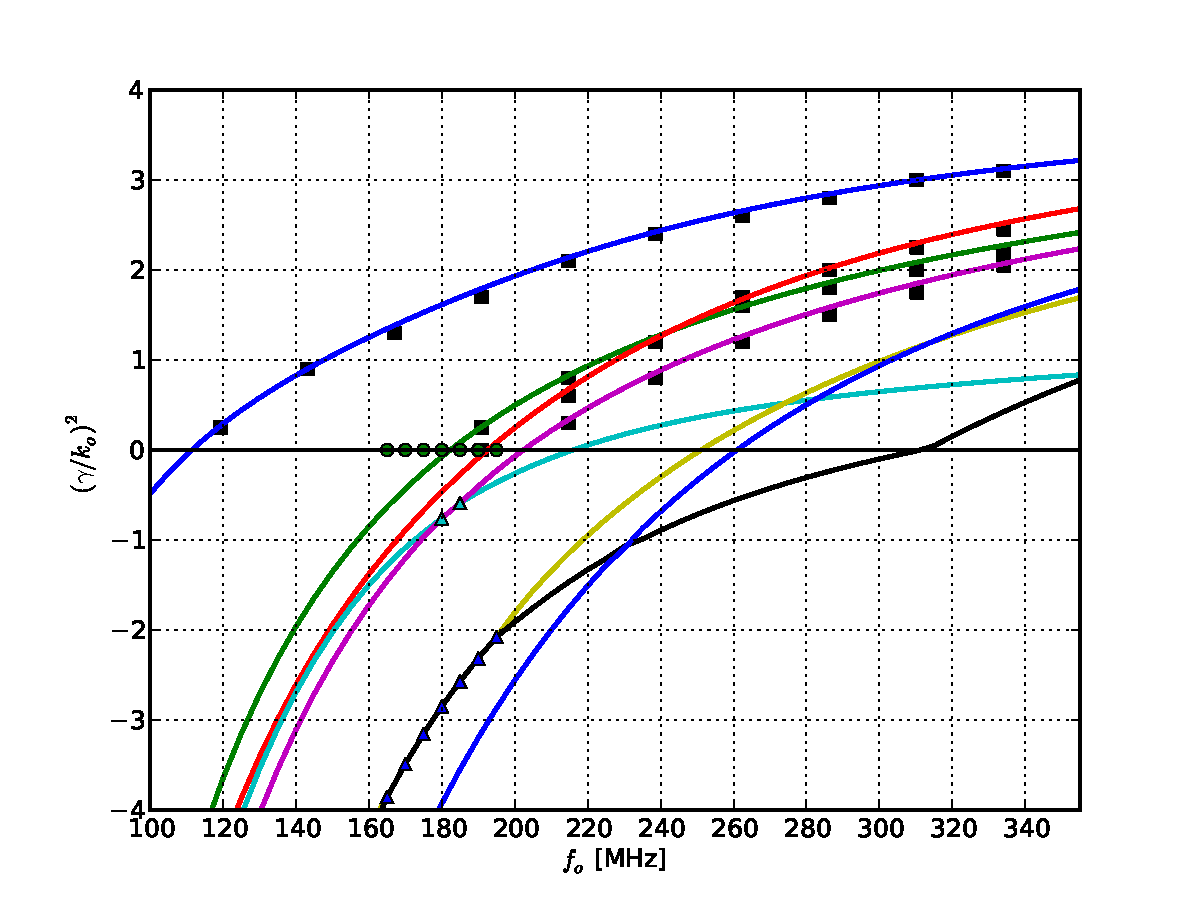
\includegraphics[width=\largefig]{chapters/lezar/pdf/half_loaded_dispersion_curve.pdf}
 \caption{Dispersion curves for the first 8 modes of a
   $1$~m~$\times~0.5$~m rectangular waveguide with its lower half
   filled with an $\epsilon_r = 4$ dielectric material.  Reference
   values for the first 4 modes from~\cite{Jin2002} are shown as
   $\blacksquare$.  The presence of complex mode pairs are indicated
   by $\blacktriangle$ and $\bullet$.}
 \index{dispersion curves}
 \label{lezar:fig:half_loaded_rectangular_dispersion_curves}
\end{figure}
\index{waveguide!half-loaded rectangular|)}
\subsection{Shielded Microstrip}
\index{shielded microstrip|(}
\index{microstrip|see{shielded microstrip}}
\label{lezar:sec:shielded_microstrip}
Microstrip line is a very popular type of planar transmission line,
primarily due to the fact that it can be constructed using
photolithographic processes and integrates easily with other microwave
components~\cite{Pozar2005}. Such a structure typically consists of a
thin conducting strip on a dielectric substrate above a ground
plane. In addition, the strip may be shielded by enclosing it in a PEC
box to reduce electromagnetic interference. A cross section of a
shielded microstrip line is shown in
Figure~\ref{lezar:fig:shielded_microstrip} with the thickness of the strip,
$t$, exaggerated for clarity. The dimensions used to obtain the
results discussed here are given in
Table~\ref{lezar:tab:shielded_microstrip_dimensions}.
\begin{figure}[t]
    \centering
    %\psfrag{epsilon}{$\epsilon_r = 1$}
    %\psfrag{mu}{$\mu_r = 1$}
    %\psfrag{edielectric}{$\epsilon_r = 8.875$}
    %\psfrag{a}{$a$}
    %\psfrag{b}{$b$}
    %\psfrag{d}{$d$}
    %\psfrag{t}{$t$}
    %\psfrag{w}{$w$}
    \resizebox{0.5\textwidth}{!}{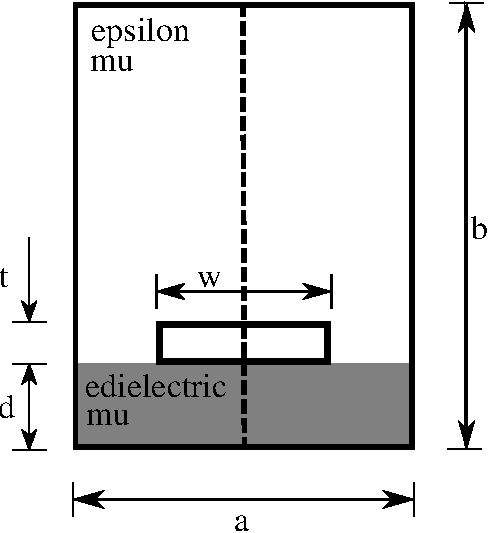
\includegraphics{chapters/lezar/pdf/shielded_microstrip_waveguide.pdf}}
    \caption{A diagram showing the cross section and dimensions of a shielded microstrip line.  The microstrip is etched on a dielectric material with a relative permittivity of $\epsilon_r = 8.75$.  The plane of symmetry is indicated by a dashed line and is modelled as a magnetic wall in order to reduce the size of the computational domain.}
    \label{lezar:fig:shielded_microstrip}
\end{figure}
\begin{table}[b]
 \centering
 \caption{Dimensions for the shielded microstrip line considered here. Definitions for the symbols are given in Figure~\ref{lezar:fig:shielded_microstrip}.}
 \label{lezar:tab:shielded_microstrip_dimensions}
 \begin{tabular}{|c|c|}
  \hline
   & Dimension [mm]\\
  \hline
   $a$, $b$ & 12.7\\
   $d$, $w$ & 1.27\\
   $t$ & 0.127\\
  \hline
 \end{tabular}
\end{table}

\paragraph{Cutoff Analysis}

Since the shielded microstrip structure consists of two conductors, it
supports a dominant transverse electromagnetic (TEM) wave that has no
axial component of the electric or magnetic field~\cite{Pozar2005}. Such
a mode has a cutoff wavenumber\index{wavenumber!cutoff} of zero and
thus propagates for all frequencies~\cite{Jin2002,PelCoc1998}. The
cutoff analysis of this structure is not considered here
explicitly. The cutoff wavenumbers for the higher order modes (which
are hybrid TE-TM modes~\cite{Pozar2005}) can however be determined from
the dispersion curves by the intersection of a curve with the
$f_o$-axis.

\paragraph{Dispersion Analysis}
\index{waveguide!dispersion analysis}

The dispersion analysis presented in~\cite{PelosiCoccioliSelleri1998} is repeated
here for validation with the resultant curves shown in
Figure~\ref{lezar:fig:shielded_microstrip_dispersion_curves}. As is the case
with the half-loaded guide, the results calculated with \fenics{}
agree well with previously published results. In the figure it is
shown that for certain parts of the frequency range of interest, modes
six and seven have complex propagation constants. Since the matrices
in the eigenvalue problem are real valued, the complex eigenvalues --
and thus the propagation constants -- must occur in complex conjugate
pairs as is the case here and reported earlier
in~\cite{HuangItoh1988}. These conjugate propagation constants are
associated with two equal modes propagating in opposite directions
along the waveguide and thus resulting in zero energy transfer. It
should be noted that for lossy materials (not considered here),
complex modes are expected but do not necessarily occur in conjugate
pairs~\cite{PelosiCoccioliSelleri1998}.
\begin{figure}[h]
 \centering
 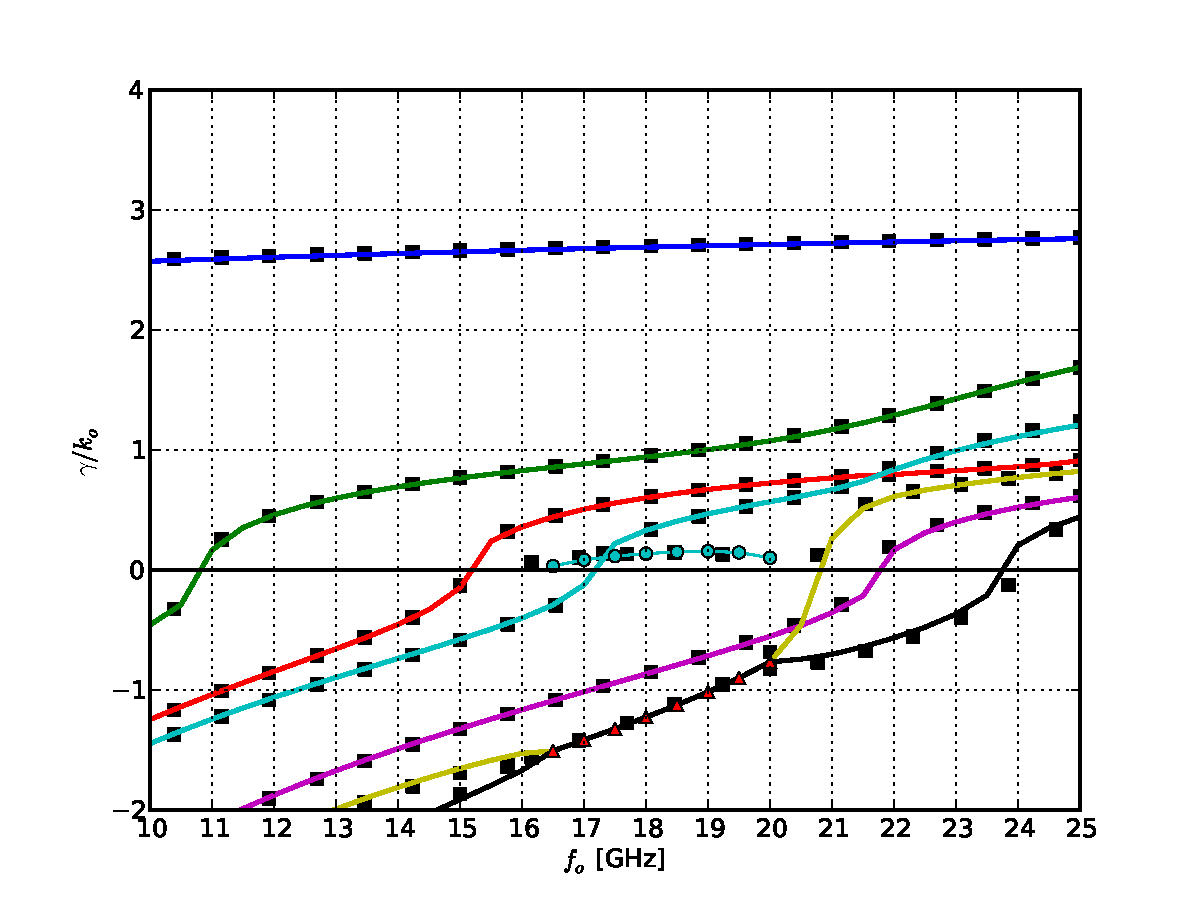
\includegraphics[width=\largefig]{chapters/lezar/pdf/shielded_microstrip_dispersion_curve.pdf}
 \caption{Dispersion curves for the first 7 even modes of shielded microstrip line using a magnetic wall to enforce symmetry.  Reference values from~\cite{PelosiCoccioliSelleri1998} are shown as $\blacksquare$.  The presence of complex mode pairs are indicated by $\blacktriangle$ and $\bullet$.}
 \index{dispersion curves}
 \label{lezar:fig:shielded_microstrip_dispersion_curves}
\end{figure}
\label{lezar:sec:shielded_microstrip|)}
\section{Analysis of Waveguide Discontinuities}
\index{waveguide!discontinuities|(}
\label{lezar:sec:waveguide_discontinuities}

Although this chapter focuses on eigenvalue type problems related to
waveguides, the use of \fenics{} in waveguide analysis is not limited
to such problems. This section briefly introduces the solution of
problems relating to waveguide discontinuities as an additional
problem class. Applications where the solutions of these problems are
of importance to microwave engineers is the design of waveguide
filters as well as the analysis and optimisation of bends in a
waveguide where properties such as the scattering parameters
(S-parameters)\index{scattering
parameters|see{S-parameters}}\index{S-parameters} of the device are
calculated~\cite{Pozar2005}.

The hybrid finite element-modal expansion technique discussed
in~\cite{PelosiCoccioliSelleri1998} is implemented and used to solve problems related
to H-plane waveguide discontinuities. For such cases -- which are
uniform in the vertical ($y$) direction transverse to the direction of
propagation ($z$) -- the problem reduces to a scalar one in two
dimensions~\cite{Jin2002} with the operating variable the
$y$-component of the electric field in the guide. In order to obtain
the scattering parameters at each port of the device, the field on the
boundary associated with the port is written as a summation of the
tangential components of the incoming and outgoing waveguide
modes. These modes can either be computed analytically, when a
junction is rectangular for example, or calculated with methods such
as those discussed in the preceding sections~\cite{MartiniPelosiSelleri2003}.

Transmission parameter (S$_{21}$) results for a length of hollow
rectangular waveguide\index{waveguide!hollow rectangular} are shown in
Figure~\ref{lezar:fig:hollow_h_plane_S_parameters}. As expected, the length
of guide behaves as a fixed value phase shifter~\cite{PelosiCoccioliSelleri1998} and
the results obtained show excellent agreement with the analytical
ones.
\begin{figure}
 \centering
 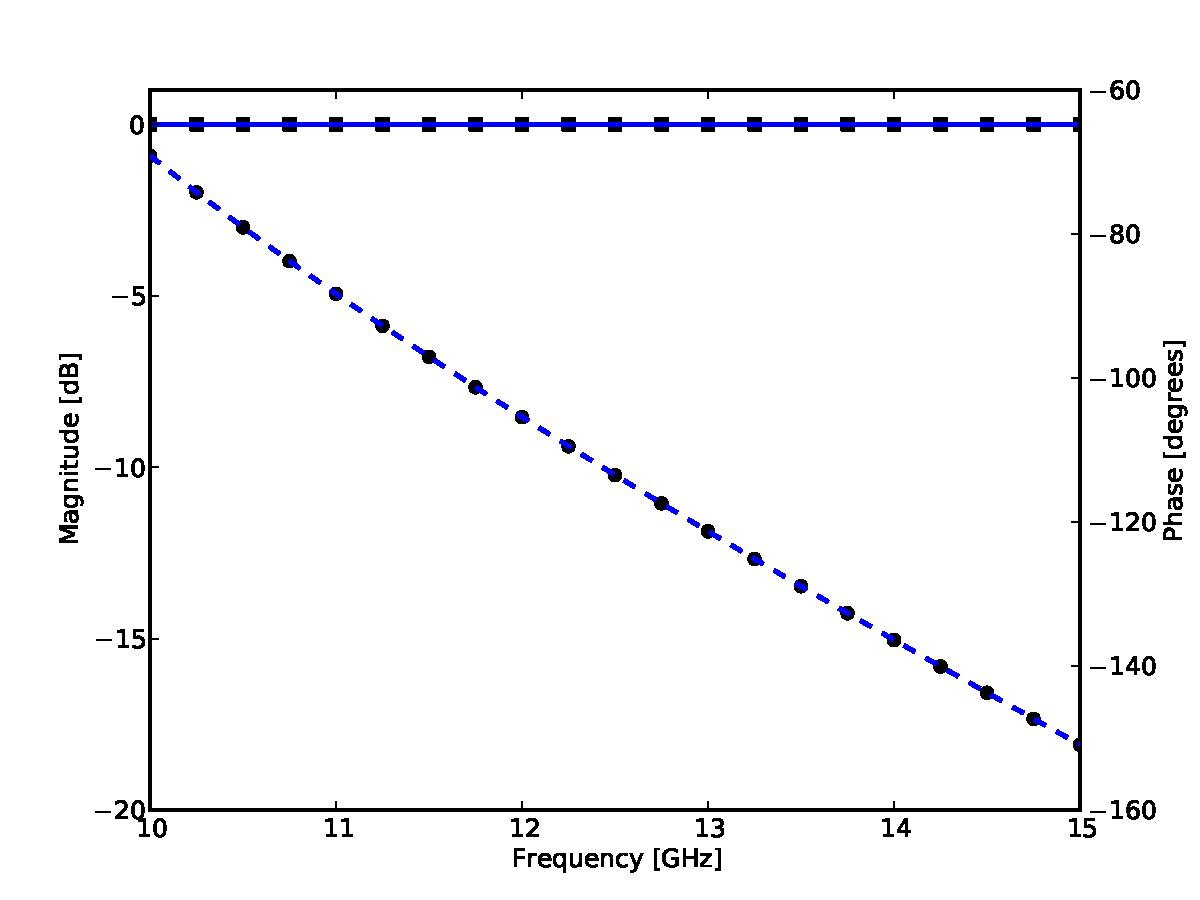
\includegraphics[width=\largefig]{chapters/lezar/pdf/hollow_h_plane_S_parameters.pdf}
 \caption{Magnitude (solid line) and phase (dashed line) of the transmission coefficient (S$_{21}$) of a length of rectangular waveguide with dimensions $a=18.35\text{mm}$, $b=9.175\text{mm}$, and $l = 10\text{mm}$. The analytical results for the same structure are indicated by markers with $\blacksquare$ and $\bullet$ indicating the magnitude and phase respectively.}
 \index{S-parameters}
 \label{lezar:fig:hollow_h_plane_S_parameters}
\end{figure}

\begin{figure}[!h]
 \centering
 %\psfrag{a}{$a$}
 %\psfrag{c}{$c$}
 %\psfrag{p}{$d$}
 %\psfrag{l}{$l$}
 %\psfrag{s}{$s$}
 %\psfrag{w}{$w$}
 %\psfrag{port1}[b1][1][1][0]{port 1}
 %\psfrag{port2}[b1][1][1][0]{port 2}
 {\resizebox{0.45\textwidth}{!}{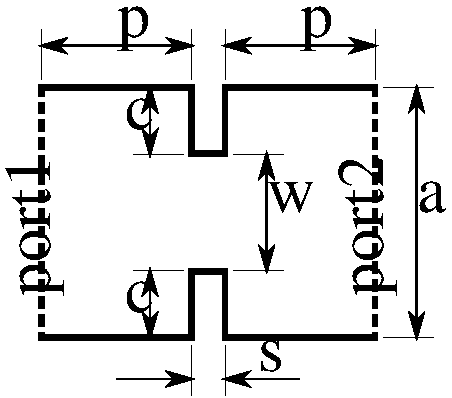
\includegraphics{chapters/lezar/pdf/h_plane_iris.pdf}}}
 \caption{Schematic of an H-plane iris in a rectangular waveguide dimensions: $a=18.35\text{mm}$, $c=4.587\text{mm}$, $d=1\text{mm}$, $s=0.5\text{mm}$, and $w=9.175\text{mm}$. The guide has a height of $b=9.175\text{mm}$. The ports are indicated by dashed lines on the boundary of the device.}
 \label{lezar:fig:h_plane_iris}
\end{figure}

A schematic for a more interesting example is the H-plane iris shown
in Figure~\ref{lezar:fig:h_plane_iris}. The figure shows the dimensions of
the structure and indicates the port definitions. The boundaries
indicated by a solid line is a PEC material. The magnitude and phase
results for the S-parameters of the device are given in
Figure~\ref{lezar:fig:h_plane_iris_S_parameters} and compared to the results
published in~\cite{PelosiCoccioliSelleri1998} with good agreement between the two
sets of data.
\begin{figure}[h]
\centering
 \subfloat[Magnitude.]{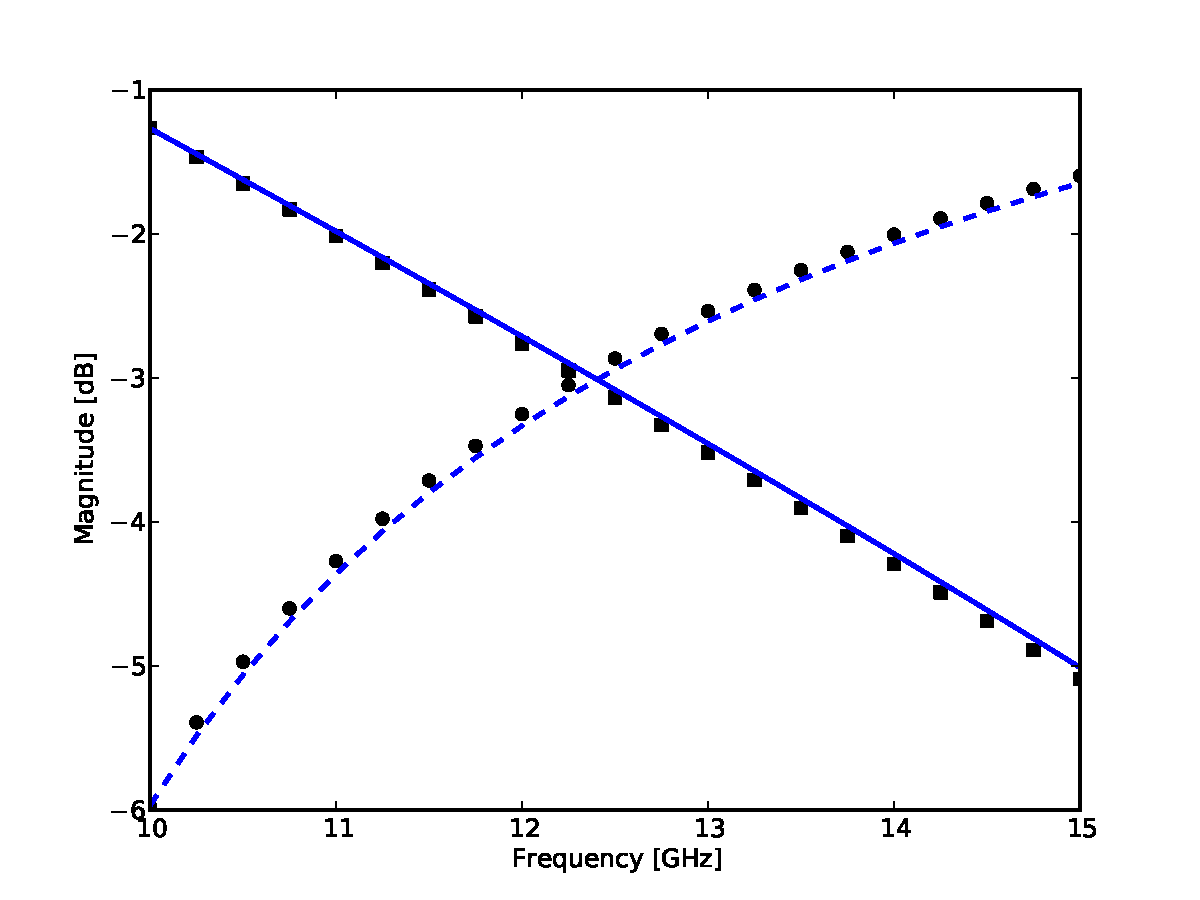
\includegraphics[width=\smallfig]{chapters/lezar/pdf/h_plane_iris_S_parameters_magnitude.pdf}}
 \subfloat[Phase.]{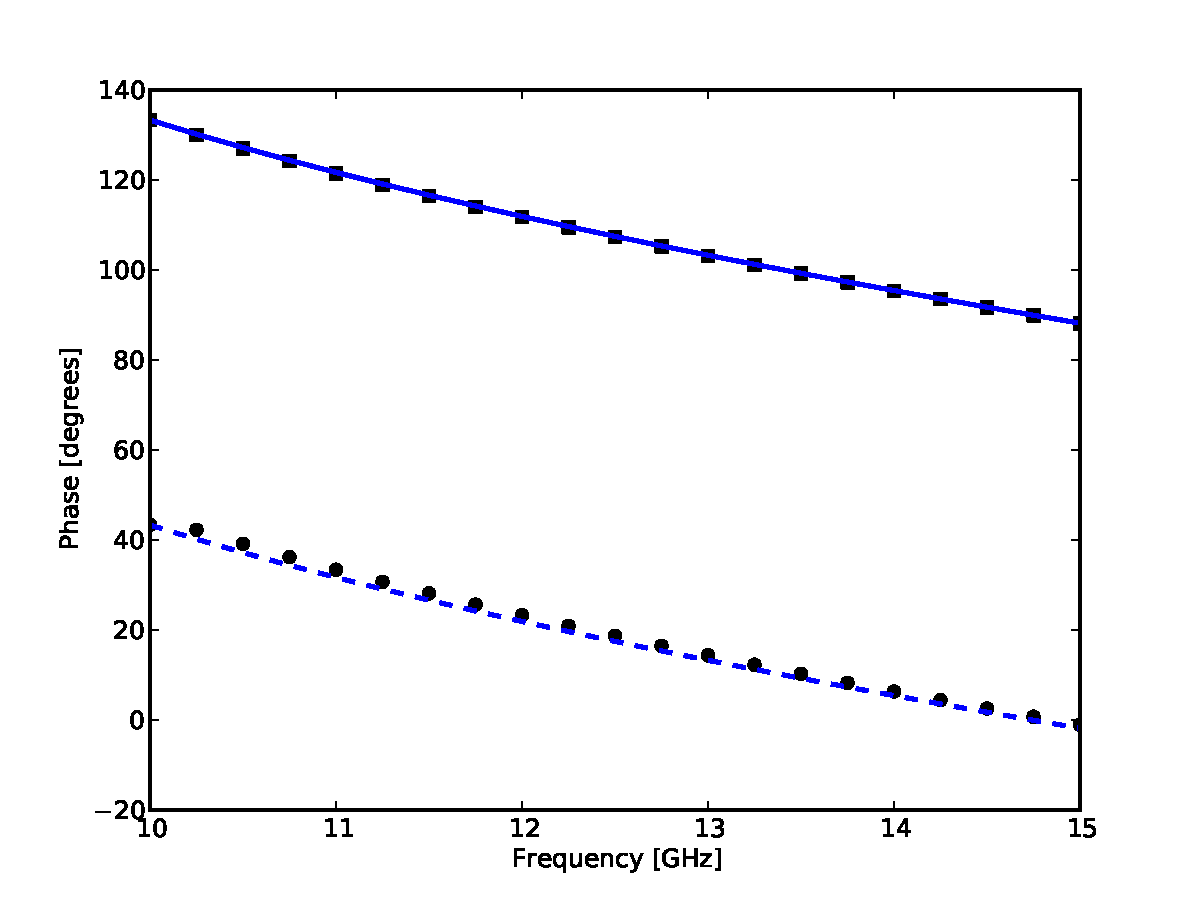
\includegraphics[width=\smallfig]{chapters/lezar/pdf/h_plane_iris_S_parameters_phase.pdf}}
 \caption{Results for the magnitude and phase of the reflection
   coefficient (S$_{11}$ -- solid line) and transmission coefficient
   (S$_{21}$ -- dashed line) of an H-plane iris in a rectangular
   waveguide shown in Figure~\ref{lezar:fig:h_plane_iris}. Reference
   results from~\cite{PelosiCoccioliSelleri1998} are indicated by markers with
   $\blacksquare$ and $\bullet$ indicating the reflection and
   transmission coefficient respectively.}
 \index{S-parameters}
 \label{lezar:fig:h_plane_iris_S_parameters}
\end{figure}
\index{waveguide!discontinuities|)}
\section{Conclusion}
In this chapter, the solutions of cutoff and dispersion problems
associated with electromagnetic waveguiding structures have been
implemented and the results analysed. In all cases, the results
obtained agree well with previously published or analytical
results. This is also the case where the analysis of waveguide
discontinuities are considered, and although the solutions shown here
are restricted to H-plane waveguide discontinuities, the methods
applied are applicable to other classes of problems such as E-plane
junctions and full 3D analysis.

This chapter has also illustrated the ease with which complex
formulations can be implemented and how quickly solutions can be
obtained. This is largely due to the almost one-to-one correspondence
between the expressions at a formulation level and the high-level code
that is used to implement a particular solution. Even in cases where
the required functionality is limited or missing, the use of \fenics{}
in conjunction with external packages greatly reduces development
time.
